% Options for packages loaded elsewhere
\PassOptionsToPackage{unicode}{hyperref}
\PassOptionsToPackage{hyphens}{url}
%
\documentclass[
  ignorenonframetext,
]{beamer}
\usepackage{pgfpages}
\setbeamertemplate{caption}[numbered]
\setbeamertemplate{caption label separator}{: }
\setbeamercolor{caption name}{fg=normal text.fg}
\beamertemplatenavigationsymbolsempty
% Prevent slide breaks in the middle of a paragraph
\widowpenalties 1 10000
\raggedbottom
\setbeamertemplate{part page}{
  \centering
  \begin{beamercolorbox}[sep=16pt,center]{part title}
    \usebeamerfont{part title}\insertpart\par
  \end{beamercolorbox}
}
\setbeamertemplate{section page}{
  \centering
  \begin{beamercolorbox}[sep=12pt,center]{part title}
    \usebeamerfont{section title}\insertsection\par
  \end{beamercolorbox}
}
\setbeamertemplate{subsection page}{
  \centering
  \begin{beamercolorbox}[sep=8pt,center]{part title}
    \usebeamerfont{subsection title}\insertsubsection\par
  \end{beamercolorbox}
}
\AtBeginPart{
  \frame{\partpage}
}
\AtBeginSection{
  \ifbibliography
  \else
    \frame{\sectionpage}
  \fi
}
\AtBeginSubsection{
  \frame{\subsectionpage}
}
\usepackage{amsmath,amssymb}
\usepackage{iftex}
\ifPDFTeX
  \usepackage[T1]{fontenc}
  \usepackage[utf8]{inputenc}
  \usepackage{textcomp} % provide euro and other symbols
\else % if luatex or xetex
  \usepackage{unicode-math} % this also loads fontspec
  \defaultfontfeatures{Scale=MatchLowercase}
  \defaultfontfeatures[\rmfamily]{Ligatures=TeX,Scale=1}
\fi
\usepackage{lmodern}
\usetheme[]{Madrid}
\ifPDFTeX\else
  % xetex/luatex font selection
\fi
% Use upquote if available, for straight quotes in verbatim environments
\IfFileExists{upquote.sty}{\usepackage{upquote}}{}
\IfFileExists{microtype.sty}{% use microtype if available
  \usepackage[]{microtype}
  \UseMicrotypeSet[protrusion]{basicmath} % disable protrusion for tt fonts
}{}
\makeatletter
\@ifundefined{KOMAClassName}{% if non-KOMA class
  \IfFileExists{parskip.sty}{%
    \usepackage{parskip}
  }{% else
    \setlength{\parindent}{0pt}
    \setlength{\parskip}{6pt plus 2pt minus 1pt}}
}{% if KOMA class
  \KOMAoptions{parskip=half}}
\makeatother
\usepackage{xcolor}
\newif\ifbibliography
\usepackage{color}
\usepackage{fancyvrb}
\newcommand{\VerbBar}{|}
\newcommand{\VERB}{\Verb[commandchars=\\\{\}]}
\DefineVerbatimEnvironment{Highlighting}{Verbatim}{commandchars=\\\{\}}
% Add ',fontsize=\small' for more characters per line
\usepackage{framed}
\definecolor{shadecolor}{RGB}{248,248,248}
\newenvironment{Shaded}{\begin{snugshade}}{\end{snugshade}}
\newcommand{\AlertTok}[1]{\textcolor[rgb]{0.94,0.16,0.16}{#1}}
\newcommand{\AnnotationTok}[1]{\textcolor[rgb]{0.56,0.35,0.01}{\textbf{\textit{#1}}}}
\newcommand{\AttributeTok}[1]{\textcolor[rgb]{0.13,0.29,0.53}{#1}}
\newcommand{\BaseNTok}[1]{\textcolor[rgb]{0.00,0.00,0.81}{#1}}
\newcommand{\BuiltInTok}[1]{#1}
\newcommand{\CharTok}[1]{\textcolor[rgb]{0.31,0.60,0.02}{#1}}
\newcommand{\CommentTok}[1]{\textcolor[rgb]{0.56,0.35,0.01}{\textit{#1}}}
\newcommand{\CommentVarTok}[1]{\textcolor[rgb]{0.56,0.35,0.01}{\textbf{\textit{#1}}}}
\newcommand{\ConstantTok}[1]{\textcolor[rgb]{0.56,0.35,0.01}{#1}}
\newcommand{\ControlFlowTok}[1]{\textcolor[rgb]{0.13,0.29,0.53}{\textbf{#1}}}
\newcommand{\DataTypeTok}[1]{\textcolor[rgb]{0.13,0.29,0.53}{#1}}
\newcommand{\DecValTok}[1]{\textcolor[rgb]{0.00,0.00,0.81}{#1}}
\newcommand{\DocumentationTok}[1]{\textcolor[rgb]{0.56,0.35,0.01}{\textbf{\textit{#1}}}}
\newcommand{\ErrorTok}[1]{\textcolor[rgb]{0.64,0.00,0.00}{\textbf{#1}}}
\newcommand{\ExtensionTok}[1]{#1}
\newcommand{\FloatTok}[1]{\textcolor[rgb]{0.00,0.00,0.81}{#1}}
\newcommand{\FunctionTok}[1]{\textcolor[rgb]{0.13,0.29,0.53}{\textbf{#1}}}
\newcommand{\ImportTok}[1]{#1}
\newcommand{\InformationTok}[1]{\textcolor[rgb]{0.56,0.35,0.01}{\textbf{\textit{#1}}}}
\newcommand{\KeywordTok}[1]{\textcolor[rgb]{0.13,0.29,0.53}{\textbf{#1}}}
\newcommand{\NormalTok}[1]{#1}
\newcommand{\OperatorTok}[1]{\textcolor[rgb]{0.81,0.36,0.00}{\textbf{#1}}}
\newcommand{\OtherTok}[1]{\textcolor[rgb]{0.56,0.35,0.01}{#1}}
\newcommand{\PreprocessorTok}[1]{\textcolor[rgb]{0.56,0.35,0.01}{\textit{#1}}}
\newcommand{\RegionMarkerTok}[1]{#1}
\newcommand{\SpecialCharTok}[1]{\textcolor[rgb]{0.81,0.36,0.00}{\textbf{#1}}}
\newcommand{\SpecialStringTok}[1]{\textcolor[rgb]{0.31,0.60,0.02}{#1}}
\newcommand{\StringTok}[1]{\textcolor[rgb]{0.31,0.60,0.02}{#1}}
\newcommand{\VariableTok}[1]{\textcolor[rgb]{0.00,0.00,0.00}{#1}}
\newcommand{\VerbatimStringTok}[1]{\textcolor[rgb]{0.31,0.60,0.02}{#1}}
\newcommand{\WarningTok}[1]{\textcolor[rgb]{0.56,0.35,0.01}{\textbf{\textit{#1}}}}
\usepackage{graphicx}
\makeatletter
\def\maxwidth{\ifdim\Gin@nat@width>\linewidth\linewidth\else\Gin@nat@width\fi}
\def\maxheight{\ifdim\Gin@nat@height>\textheight\textheight\else\Gin@nat@height\fi}
\makeatother
% Scale images if necessary, so that they will not overflow the page
% margins by default, and it is still possible to overwrite the defaults
% using explicit options in \includegraphics[width, height, ...]{}
\setkeys{Gin}{width=\maxwidth,height=\maxheight,keepaspectratio}
% Set default figure placement to htbp
\makeatletter
\def\fps@figure{htbp}
\makeatother
\setlength{\emergencystretch}{3em} % prevent overfull lines
\providecommand{\tightlist}{%
  \setlength{\itemsep}{0pt}\setlength{\parskip}{0pt}}
\setcounter{secnumdepth}{-\maxdimen} % remove section numbering
\logo{
\includegraphics[height=1cm,width=3cm]{logo.png}}
\usetheme{Madrid}
\usefonttheme{serif}
\setbeamertemplate{navigation symbols}{}
\usepackage{lmodern}  % for bold teletype font
\usepackage{amsmath}  % for \hookrightarrow
\usepackage{xcolor}   % for \textcolor


\ifLuaTeX
  \usepackage{selnolig}  % disable illegal ligatures
\fi
\IfFileExists{bookmark.sty}{\usepackage{bookmark}}{\usepackage{hyperref}}
\IfFileExists{xurl.sty}{\usepackage{xurl}}{} % add URL line breaks if available
\urlstyle{same}
\hypersetup{
  pdftitle={Leksioni 5},
  pdfauthor={Endri Raco},
  hidelinks,
  pdfcreator={LaTeX via pandoc}}

\title{Leksioni 5}
\author{Endri Raco}
\date{28 April, 2024}

\begin{document}
\frame{\titlepage}

\begin{frame}[allowframebreaks]
  \tableofcontents[hideallsubsections]
\end{frame}
\hypertarget{analiza-gjeografike-e-tuxeb-dhuxebnave-me-python}{%
\section{Analiza Gjeografike e të Dhënave me
Python}\label{analiza-gjeografike-e-tuxeb-dhuxebnave-me-python}}

\begin{frame}{Analiza Gjeografike e të Dhënave me Python}
\protect\hypertarget{analiza-gjeografike-e-tuxeb-dhuxebnave-me-python-1}{}
\begin{itemize}
\item
  Do të mësoni se si të integrohen të dhënat gjeohapësinore në rrjedhën
  tuaj të punës me Python për analizën e të dhënave.
\item
  Para se të hyjmë në manipulimin dhe analizimin e të dhënave
  hapësinore, le të ndalemi një moment dhe të përcaktojmë çfarë
  saktësisht janë të dhënat gjeohapësinore.
\end{itemize}
\end{frame}

\begin{frame}{Çfarë janë të Dhënat Gjeohapësinore?}
\protect\hypertarget{uxe7faruxeb-januxeb-tuxeb-dhuxebnat-gjeohapuxebsinore}{}
\begin{itemize}
\item
  Të dhënat gjeohapësinore janë të dhëna për të cilat një vendndodhje
  specifike është e lidhur me secilin rekord.
\item
  Së pari, këto janë të dhëna.
\item
  Shumë nga operacionet që do të bëjmë me të dhënat gjeohapësinore janë
  shumë të ngjashme me ato që do të bënim me të dhënat jo-hapësinore.
\end{itemize}
\end{frame}

\begin{frame}{Të Dhënat Gjeohapësinore}
\protect\hypertarget{tuxeb-dhuxebnat-gjeohapuxebsinore}{}
\begin{itemize}
\item
  Por me të dhënat gjeohapësinore, çdo vrojtim ka një vendndodhje dhe
  mund të ``vendoset në një hartë''.
\item
  Kjo na lejon të shikojmë marrëdhëniet hapësinore mes të dhënave.
\item
  Forca e vërtetë e të Dhënave Gjeohapësinore është aftësia për të
  kombinuar si vetë të dhënat, ashtu edhe vendndodhjen e tyre, duke
  hapur mundësi të shumta për analiza të sofistikuara.
\end{itemize}
\end{frame}

\begin{frame}{Të Dhënat Hapësinore I}
\protect\hypertarget{tuxeb-dhuxebnat-hapuxebsinore-i}{}
\begin{itemize}
\item
  Të dhënat hapësinore vijnë në të gjitha format dhe madhësitë.
\item
  Një shembull tipik i të dhënave tradicionale gjeohapësinore janë të
  dhënat e regjistrimit qeveritar.
\end{itemize}
\end{frame}

\begin{frame}{Të Dhënat Hapësinore I}
\protect\hypertarget{tuxeb-dhuxebnat-hapuxebsinore-i-1}{}
Këtu, ne shohim një imazh të dendësisë së popullsisë në Shtetet e
Bashkuara.

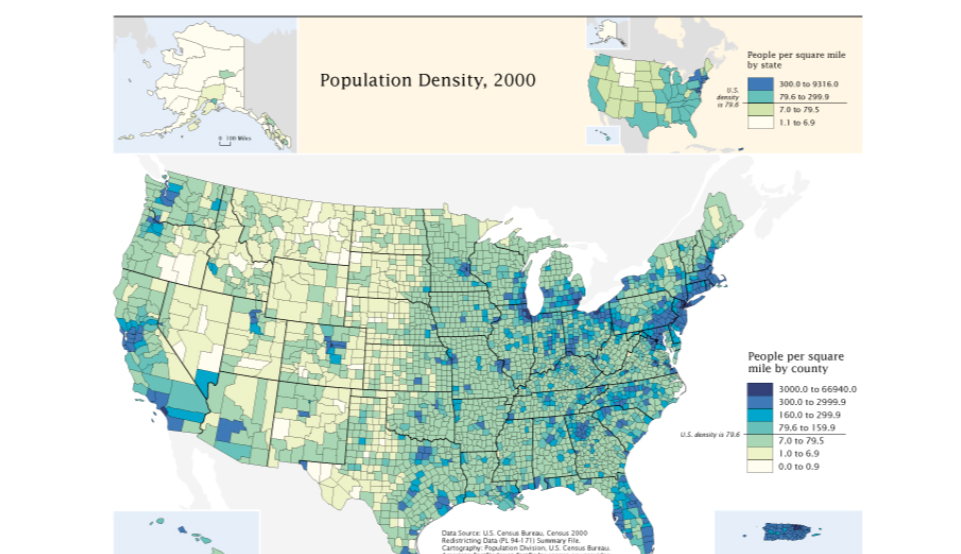
\includegraphics{./Figs/census1.png}
\end{frame}

\begin{frame}{Të Dhënat Hapësinore II}
\protect\hypertarget{tuxeb-dhuxebnat-hapuxebsinore-ii}{}
\begin{itemize}
\tightlist
\item
  Kohët e fundit, ka një disponueshmëri në rritje e burimeve të reja të
  të dhënave hapësinore.
\end{itemize}
\end{frame}

\begin{frame}{Si e regjistrojmë botën reale}
\protect\hypertarget{si-e-regjistrojmuxeb-botuxebn-reale}{}
\begin{itemize}
\tightlist
\item
  Në GIS, ka dy modele të të dhënave për mënyrën se si e regjistrojmë
  botën.
\end{itemize}

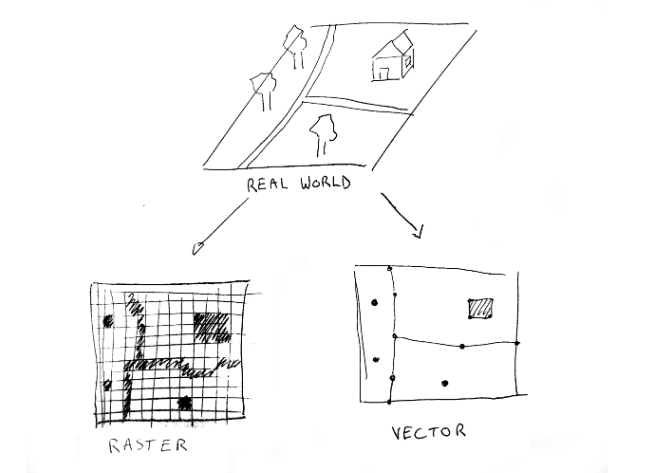
\includegraphics{./Figs/rasvec.png} \#\# Si e regjistrojmë botën reale

\begin{itemize}
\item
  Modeli i parë është një \textbf{raster}, i cili kodon botën si një
  sipërfaqe të vazhdueshme të përfaqësuar nga një rrjetë, si p.sh.
  piksela të një imazhi.
\item
  Shembuj përfshijnë të dhënat e lartësisë ose imazhet nga sateliti.
\end{itemize}
\end{frame}

\begin{frame}{Si e regjistrojmë botën reale}
\protect\hypertarget{si-e-regjistrojmuxeb-botuxebn-reale-1}{}
\begin{itemize}
\item
  Modeli tjetër është të përfaqësojmë botën si një koleksion objektesh
  të ndara duke përdorur pika, linja dhe poligone.
\item
  Këto quhen të dhëna vektoriale.
\end{itemize}
\end{frame}

\begin{frame}{Raster vs.~të dhënave vektoriale}
\protect\hypertarget{raster-vs.-tuxeb-dhuxebnave-vektoriale}{}
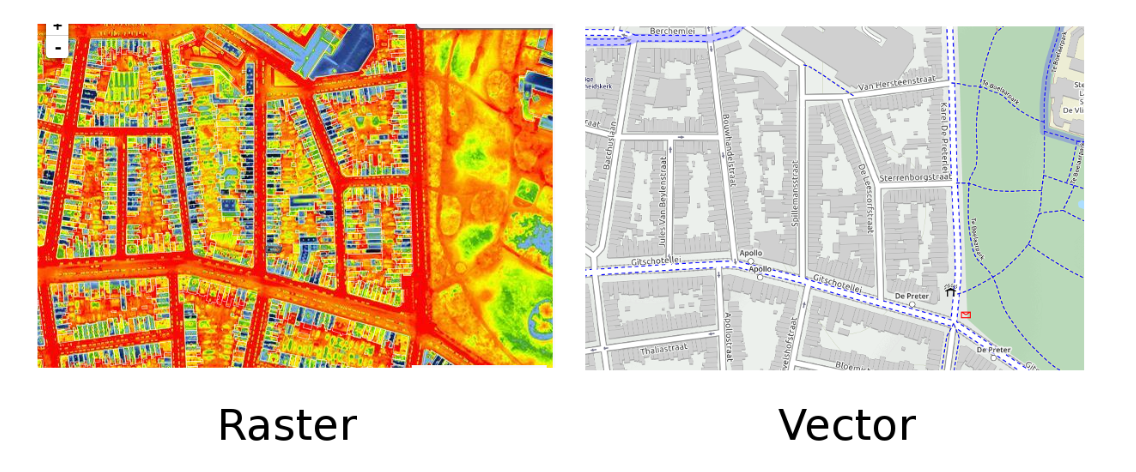
\includegraphics{./Figs/rasvec2.png} \#\# Raster vs.~të dhënave
vektoriale

\begin{itemize}
\item
  Këtu është një shembull real i dy modeleve të të dhënave të së njëjtës
  zonë.
\item
  Në anën e majtë, shohim një imazh satelitor termik që tregon humbjen e
  ngrohtësisë së ndërtesave.
\item
  Në anën e djathtë, sohim një vizualizim të të dhënave vektoriale të së
  njëjtës zonë: karakteristika të veçanta ku ndërtesat janë të
  përfaqësuara si poligone dhe rrugët si linja.
\end{itemize}
\end{frame}

\begin{frame}{Karakteristikat vektoriale}
\protect\hypertarget{karakteristikat-vektoriale}{}
\begin{itemize}
\tightlist
\item
  Karakteristikat vektoriale përbëhen nga tre lloje të ndryshme të
  gjeometrive:
\end{itemize}
\end{frame}

\begin{frame}{Karakteristikat vektoriale}
\protect\hypertarget{karakteristikat-vektoriale-1}{}
\begin{itemize}
\tightlist
\item
  Fillimisht, kemi një gjeometri pikash \textbf{point}: një vendndodhje
  e vetme me koordinata X dhe Y.
\end{itemize}

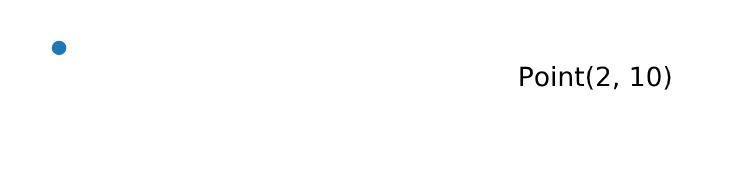
\includegraphics{./Figs/point.png}
\end{frame}

\begin{frame}{Karakteristikat vektoriale}
\protect\hypertarget{karakteristikat-vektoriale-2}{}
\begin{itemize}
\tightlist
\item
  Tjetra, një vijë \textbf{line} është një grup pikash të lidhura.
\end{itemize}

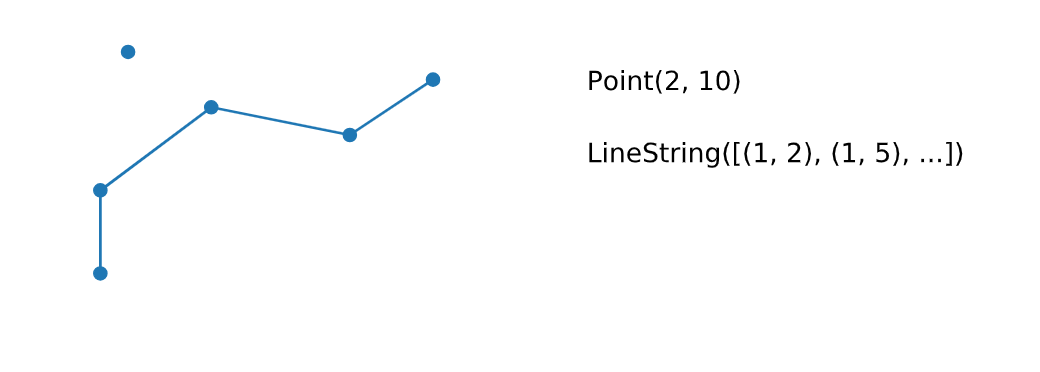
\includegraphics{./Figs/line.png}

\begin{itemize}
\tightlist
\item
  Në kod, do të vëreni se kjo quhet ``linestring''.
\end{itemize}
\end{frame}

\begin{frame}{Karakteristikat vektoriale}
\protect\hypertarget{karakteristikat-vektoriale-3}{}
\begin{itemize}
\tightlist
\item
  Së fundmi, një poligon \textbf{polygon} formohet nga një vijë e
  mbyllur që rrethon një zonë.
\end{itemize}

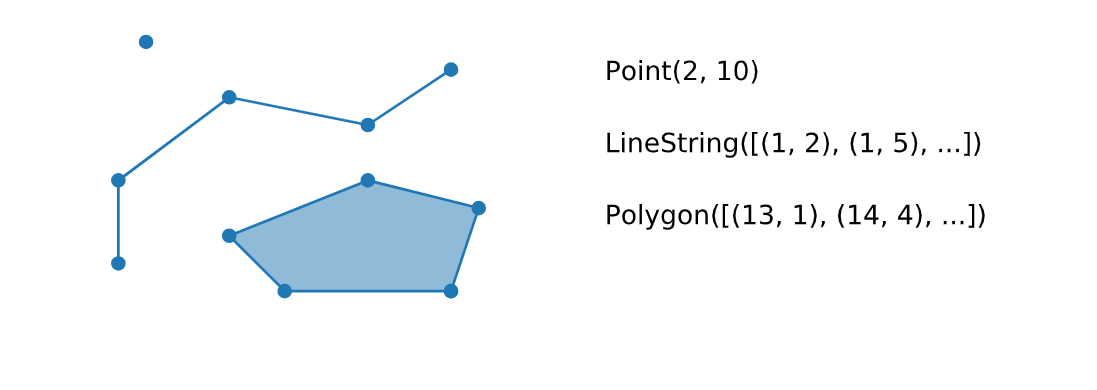
\includegraphics{./Figs/polygon.png}

\begin{itemize}
\tightlist
\item
  Përveç kësaj, një karakteristikë mund të përbëhet edhe nga disa
  gjeometri të ndryshme, siç është një ``MultiPolygon''.
\end{itemize}
\end{frame}

\begin{frame}{Shembull vektorial I}
\protect\hypertarget{shembull-vektorial-i}{}
Le të japim një shembull real që ilustron ato lloje të të dhënave
vektoriale: ne mund të visualizojmë vendet e botës si poligone, të
treguara këtu në këtë figurë.

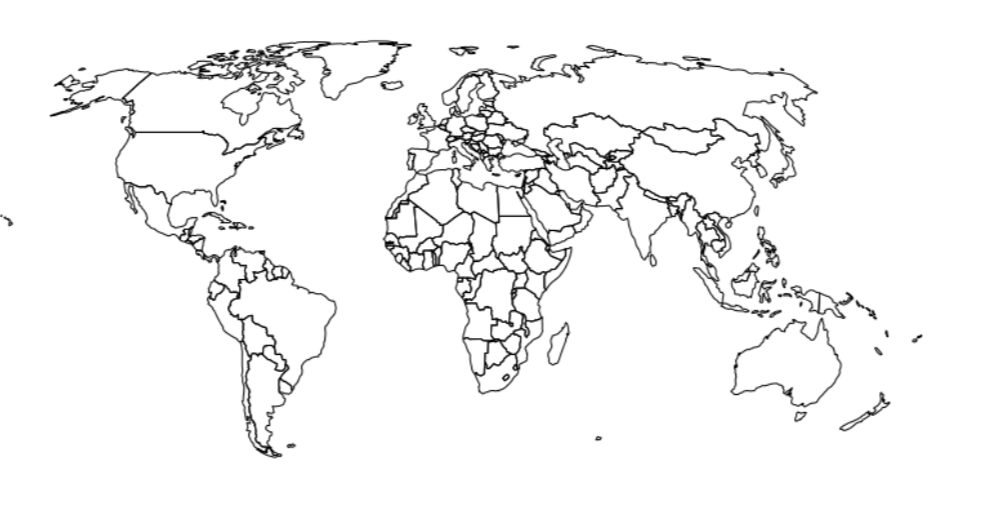
\includegraphics{./Figs/world.png}
\end{frame}

\begin{frame}{Shembull vektorial II}
\protect\hypertarget{shembull-vektorial-ii}{}
Tani shtojmë vendndodhjet e kryeqyteteve si karakteristika pikash.

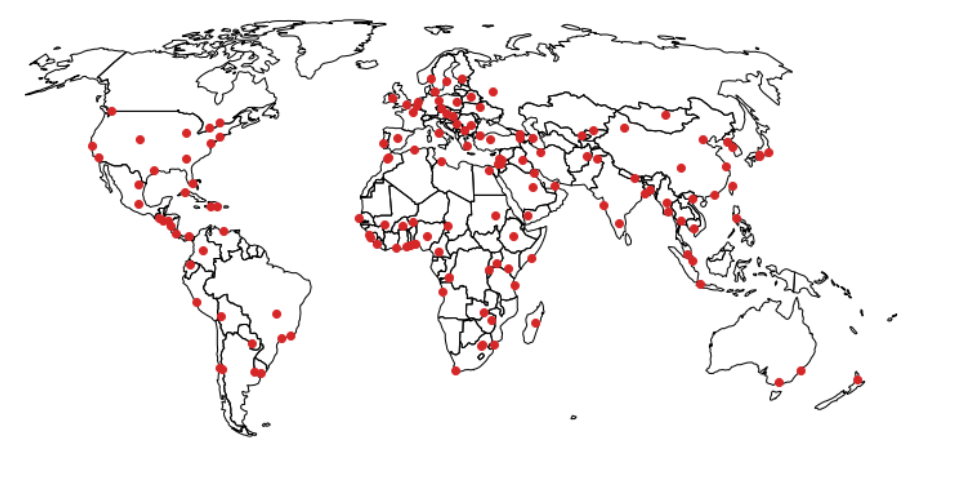
\includegraphics{./Figs/capital.png}
\end{frame}

\begin{frame}{Shembull vektorial III}
\protect\hypertarget{shembull-vektorial-iii}{}
Së fundmi, shtojmë disa nga lumenjtë më të mëdhenj të botës si linja.

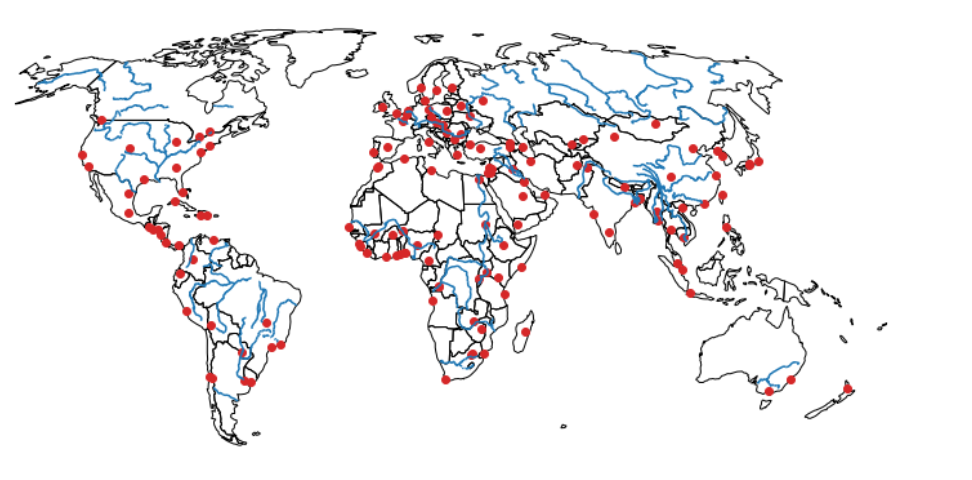
\includegraphics{./Figs/capline.png}
\end{frame}

\begin{frame}{Të dhënat e atributeve vektoriale}
\protect\hypertarget{tuxeb-dhuxebnat-e-atributeve-vektoriale}{}
\begin{itemize}
\item
  Një koncept i rëndësishëm janë atributet e karakteristikave.
\item
  Zakonisht, ne do të kemi informacion mbi karakteristikat tona
  vektoriale.
\end{itemize}
\end{frame}

\begin{frame}{Të dhënat e atributeve vektoriale}
\protect\hypertarget{tuxeb-dhuxebnat-e-atributeve-vektoriale-1}{}
\begin{itemize}
\item
  Duke përdorur poligonet e vendeve si shembull, mund të kemi
  informacion mbi emrin e vendit, kryeqytetin e tij, numrin e
  popullsisë, etj.
\item
  Kur kemi një koleksion të tillë karakteristikash, për shembull, të
  gjitha vendet në botë, të kombinuara me atributet e tij, përfundojmë
  me një tabelë.
\end{itemize}

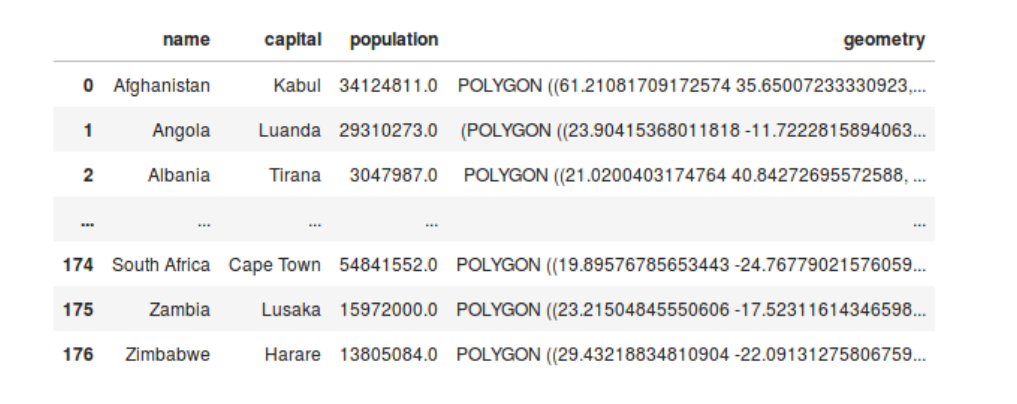
\includegraphics{./Figs/geotable.png}

Ky është lloji i të dhënave që do të përdoret në këtë kurs.
\end{frame}

\begin{frame}{Le të praktikojmë!}
\protect\hypertarget{le-tuxeb-praktikojmuxeb}{}
\begin{itemize}
\item
  Për ushtrimet, do përdorim njohuritë bazë nga pandas për të punuar me
  të dhënat tabelare, dhe matplotlib për vizualizimin.
\item
  Le të bëjmë disa ushtrime të para duke përdorur këto paketa.
\end{itemize}
\end{frame}

\begin{frame}{Shembull: Restorantet në Paris}
\protect\hypertarget{shembull-restorantet-nuxeb-paris}{}
\begin{itemize}
\item
  Në këtë ushtrim, do të punojmë me një dataset që përmban të dhëna mbi
  restorantet në qendrën e Parisit.
\item
  Do të përdorim pandas për të lexuar të dhënat nga një skedar CSV dhe
  matplotlib për të krijuar një vizualizim të thjeshtë të koordinatave
  ````të restoranteve.
\end{itemize}
\end{frame}

\begin{frame}[fragile]{Importimi i bibliotekave}
\protect\hypertarget{importimi-i-bibliotekave}{}
\AddToHookNext{env/Highlighting/begin}{\scriptsize}

\begin{Shaded}
\begin{Highlighting}[]
\ImportTok{import}\NormalTok{ pandas }\ImportTok{as}\NormalTok{ pd}
\ImportTok{import}\NormalTok{ matplotlib.pyplot }\ImportTok{as}\NormalTok{ plt}
\end{Highlighting}
\end{Shaded}
\end{frame}

\begin{frame}[fragile]{Leximi i datasetit}
\protect\hypertarget{leximi-i-datasetit}{}
\AddToHookNext{env/Highlighting/begin}{\scriptsize}

\begin{Shaded}
\begin{Highlighting}[]
\CommentTok{\# Lexojmë skedarin CSV që përmban të dhënat e restoranteve}
\NormalTok{restaurants }\OperatorTok{=}\NormalTok{ pd.read\_csv(}\StringTok{"data/gis/paris\_restaurants.csv"}\NormalTok{)}
\end{Highlighting}
\end{Shaded}
\end{frame}

\begin{frame}[fragile]{Inspektimi i të dhënave}
\protect\hypertarget{inspektimi-i-tuxeb-dhuxebnave}{}
\AddToHookNext{env/Highlighting/begin}{\scriptsize}

\begin{Shaded}
\begin{Highlighting}[]
\CommentTok{\# Shikojmë 5 rreshtat e parë të datasetit për të parë strukturën e tij}
\BuiltInTok{print}\NormalTok{(restaurants.head())}
\end{Highlighting}
\end{Shaded}

Kjo do të na tregojë nëse kemi kolona me koordinata X dhe Y që
përfaqësojnë vendndodhjet e restoranteve.
\end{frame}

\begin{frame}[fragile]{Vizualizimi i vendndodhjeve të restoranteve}
\protect\hypertarget{vizualizimi-i-vendndodhjeve-tuxeb-restoranteve}{}
\AddToHookNext{env/Highlighting/begin}{\scriptsize}

\begin{Shaded}
\begin{Highlighting}[]
\CommentTok{\# Krijojmë një figurë dhe një aks me matplotlib}
\NormalTok{fig, ax }\OperatorTok{=}\NormalTok{ plt.subplots()}

\CommentTok{\# Përdorim metodën plot() për të vizualizuar vendndodhjet e restoranteve}
\CommentTok{\# Ne përdorim kolonat që përmbajnë koordinatat X dhe Y për të krijuar grafikun}
\NormalTok{ax.plot(restaurants[}\StringTok{"x"}\NormalTok{], restaurants[}\StringTok{"y"}\NormalTok{], }\StringTok{\textquotesingle{}o\textquotesingle{}}\NormalTok{, color }\OperatorTok{=} \StringTok{"Blue"}\NormalTok{)  }\CommentTok{\# \textquotesingle{}o\textquotesingle{} për pikë të vetme}

\CommentTok{\# Shtohet një titull për grafikun}
\NormalTok{ax.set\_title(}\StringTok{"Vendndodhjet e Restoranteve në Qendrën e Parisit"}\NormalTok{)}

\CommentTok{\# Tregojmë grafikun}
\NormalTok{plt.show()}
\end{Highlighting}
\end{Shaded}
\end{frame}

\begin{frame}{Shembull: Shtimi i Hartës së Sfondit}
\protect\hypertarget{shembull-shtimi-i-hartuxebs-suxeb-sfondit}{}
\begin{itemize}
\item
  Tani do të mësojmë si të shtojmë një hartë sfondi në vizualizimin tonë
  për të dhënë kontekst hapësinor.
\item
  Për ta bërë këtë, do të përdorim paketën \textbf{contextily} dhe
  funksionin \textbf{add\_basemap()} për të shtuar një hartë web në
  grafikun tonë.
\end{itemize}
\end{frame}

\begin{frame}[fragile]{Instalimi i contextily}
\protect\hypertarget{instalimi-i-contextily}{}
\AddToHookNext{env/Highlighting/begin}{\scriptsize}

\begin{Shaded}
\begin{Highlighting}[]
\NormalTok{conda install contextily}
\end{Highlighting}
\end{Shaded}
\end{frame}

\begin{frame}[fragile]{Importimi i contextily}
\protect\hypertarget{importimi-i-contextily}{}
\AddToHookNext{env/Highlighting/begin}{\scriptsize}

\begin{Shaded}
\begin{Highlighting}[]
\ImportTok{import}\NormalTok{ contextily }\ImportTok{as}\NormalTok{ ctx}
\end{Highlighting}
\end{Shaded}
\end{frame}

\begin{frame}[fragile]{Krijimi i vizualizimit me harten e sfondit}
\protect\hypertarget{krijimi-i-vizualizimit-me-harten-e-sfondit}{}
\AddToHookNext{env/Highlighting/begin}{\scriptsize}

\begin{Shaded}
\begin{Highlighting}[]
\CommentTok{\# Krijojmë një figurë dhe një aks me matplotlib}
\NormalTok{fig, ax }\OperatorTok{=}\NormalTok{ plt.subplots()}

\CommentTok{\# Bëjmë një grafikun e të gjitha pikave në datasetin "restaurants" me madhësi të zvogëluar}
\NormalTok{ax.plot(restaurants[}\StringTok{"x"}\NormalTok{], restaurants[}\StringTok{"y"}\NormalTok{], }\StringTok{\textquotesingle{}o\textquotesingle{}}\NormalTok{, markersize}\OperatorTok{=}\DecValTok{1}\NormalTok{)  }\CommentTok{\# Përdorim \textquotesingle{}o\textquotesingle{} për të treguar një pikë të vetme}

\CommentTok{\# Shtojmë një titull për grafikun}
\NormalTok{ax.set\_title(}\StringTok{"Vendndodhjet e Restoranteve në Qendrën e Parisit me Hartë të Sfondit"}\NormalTok{)}

\CommentTok{\# Shtojmë hartën e sfondit me contextily}
\NormalTok{ctx.add\_basemap(ax, source}\OperatorTok{=}\NormalTok{ctx.providers.OpenStreetMap.Mapnik)}

\CommentTok{\# Tregojmë grafikun}
\NormalTok{plt.show()}
\end{Highlighting}
\end{Shaded}
\end{frame}

\hypertarget{hyrje-nuxeb-geopandas}{%
\section{Hyrje në GeoPandas}\label{hyrje-nuxeb-geopandas}}

\begin{frame}{Prezantimi i GeoPandas}
\protect\hypertarget{prezantimi-i-geopandas}{}
\begin{itemize}
\tightlist
\item
  Fillojmë të prezantojmë bibliotekat specifike të Python për të dhënat
  hapësinore.
\end{itemize}
\end{frame}

\begin{frame}{Formatet e të dhënave hapësinore specifike}
\protect\hypertarget{formatet-e-tuxeb-dhuxebnave-hapuxebsinore-specifike}{}
\begin{itemize}
\item
  Në ushtrimin e fundit, përdorëm pandas për të lexuar një skedar CSV me
  koordinatat e pikave dhe përdorëm matplotlib për të krijuar një hartë
  të atyre pikave.
\item
  Megjithatë, thamë se përveç të dhënave të pikave, të dhënat hapësinore
  mund të përbëhen nga linja ose poligone.
\item
  Çdo objekt atëherë përbëhet nga disa pika, dhe për këtë arsye, nuk do
  të mund ta përfaqësojmë lehtësisht këtë në një skedar CSV ose në një
  DataFrame me dy kolona për koordinatat x dhe y.
\end{itemize}
\end{frame}

\begin{frame}{Formatet e të dhënave hapësinore specifike}
\protect\hypertarget{formatet-e-tuxeb-dhuxebnave-hapuxebsinore-specifike-1}{}
\begin{itemize}
\item
  Prandaj, më tutje, do të përdorim formate specifike për të dhënat
  gjeohapësinore, si skedarët GeoJSON, GeoPackage, ose shapefiles, të
  cilët janë të specializuar për të ruajtur të dhënat hapësinore, përveç
  të dhënave tabelare tradicionale.
\item
  Për të lexuar skedarët e tillë dhe për të punuar me të dhënat
  gjeohapësinore në Python, do të përdorim bibliotekën
  \textbf{GeoPandas}.
\end{itemize}
\end{frame}

\begin{frame}{Importimi i të dhënave gjeohapësinore me GeoPandas}
\protect\hypertarget{importimi-i-tuxeb-dhuxebnave-gjeohapuxebsinore-me-geopandas}{}
\begin{itemize}
\item
  GeoPandas është një bibliotekë për të punuar me të dhënat
  gjeohapësinore tabelare, duke zgjeruar pandas DataFrame.
\item
  Fillojmë me importimin e disa të dhënave.
\end{itemize}
\end{frame}

\begin{frame}{Importimi i të dhënave gjeohapësinore me GeoPandas}
\protect\hypertarget{importimi-i-tuxeb-dhuxebnave-gjeohapuxebsinore-me-geopandas-1}{}
\begin{itemize}
\item
  Mund të përdorim funksionin ``read\_file'' të GeoPandas, ku argument
  kemi path-in e skedarit.
\item
  Ky funksion mund të lexojë shumicën e formateve të zakonshme të të
  dhënave hapësinore.
\end{itemize}
\end{frame}

\begin{frame}[fragile]{Krijimi i vizualizimit me harten e sfondit}
\protect\hypertarget{krijimi-i-vizualizimit-me-harten-e-sfondit-1}{}
\AddToHookNext{env/Highlighting/begin}{\scriptsize}

\begin{Shaded}
\begin{Highlighting}[]
\ImportTok{import}\NormalTok{ geopandas}
\NormalTok{countries }\OperatorTok{=}\NormalTok{ geopandas.read\_file(}\StringTok{"data/gis/countries.geojson"}\NormalTok{)}
\end{Highlighting}
\end{Shaded}
\end{frame}

\begin{frame}{Krijimi i vizualizimit me harten e sfondit}
\protect\hypertarget{krijimi-i-vizualizimit-me-harten-e-sfondit-2}{}
\begin{itemize}
\item
  Në këtë shembull, po lexojmë një skedar GeoJSON me të gjitha vendet e
  botës.
\item
  Duke përdorur metodën ``head'' për të shfaqur pesë rreshtat e parë,
  mund të shihni se tani kemi një kolonë me gjeometrinë, në këtë rast
  poligone që përfaqësojnë vendet.
\item
  Dhe kolonat e tjera janë atributet që përshkruajnë ato vende.
\end{itemize}
\end{frame}

\begin{frame}[fragile]{Krijimi i vizualizimit me harten e sfondit}
\protect\hypertarget{krijimi-i-vizualizimit-me-harten-e-sfondit-3}{}
\AddToHookNext{env/Highlighting/begin}{\scriptsize}

\begin{Shaded}
\begin{Highlighting}[]
\NormalTok{countries.head()}
\end{Highlighting}
\end{Shaded}
\end{frame}

\begin{frame}{Vizualizimi i shpejtë i të dhënave hapësinore me
GeoPandas}
\protect\hypertarget{vizualizimi-i-shpejtuxeb-i-tuxeb-dhuxebnave-hapuxebsinore-me-geopandas}{}
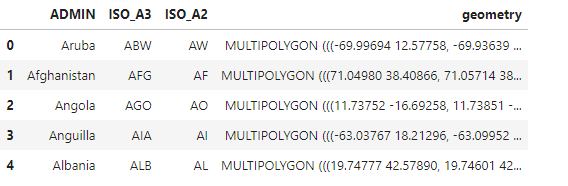
\includegraphics{./Figs/countries.png}
\end{frame}

\begin{frame}{Vizualizimi i shpejtë i të dhënave hapësinore me
GeoPandas}
\protect\hypertarget{vizualizimi-i-shpejtuxeb-i-tuxeb-dhuxebnave-hapuxebsinore-me-geopandas-1}{}
\begin{itemize}
\item
  Le të bëjmë një vizualizim të shpejtë të të dhënave për të parë që me
  të vërtetë kemi të gjitha vendet e botës.
\item
  Për këtë, mund të përdorim metodën ``plot'', e cila do të krijojë një
  vizualizim bazë të gjeometrisë së datasetit të vendeve.
\end{itemize}
\end{frame}

\begin{frame}[fragile]{Vizualizimi i shpejtë i të dhënave hapësinore me
GeoPandas}
\protect\hypertarget{vizualizimi-i-shpejtuxeb-i-tuxeb-dhuxebnave-hapuxebsinore-me-geopandas-2}{}
\AddToHookNext{env/Highlighting/begin}{\scriptsize}

\begin{Shaded}
\begin{Highlighting}[]
\NormalTok{countries.plot()}
\end{Highlighting}
\end{Shaded}
\end{frame}

\begin{frame}{Vizualizimi i shpejtë i të dhënave hapësinore me
GeoPandas}
\protect\hypertarget{vizualizimi-i-shpejtuxeb-i-tuxeb-dhuxebnave-hapuxebsinore-me-geopandas-3}{}
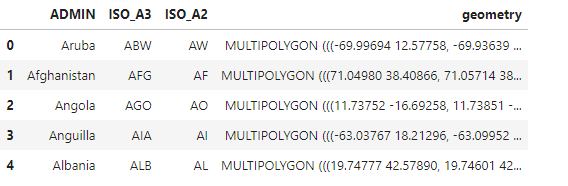
\includegraphics{./Figs/countries.png}
\end{frame}

\begin{frame}[fragile]{GeoDataFrame}
\protect\hypertarget{geodataframe}{}
\begin{itemize}
\tightlist
\item
  Por çfarë është ky objekt ``countries''?
\end{itemize}

\AddToHookNext{env/Highlighting/begin}{\scriptsize}

\begin{Shaded}
\begin{Highlighting}[]
\BuiltInTok{type}\NormalTok{(countries)}
\end{Highlighting}
\end{Shaded}
\end{frame}

\begin{frame}{GeoDataFrame}
\protect\hypertarget{geodataframe-1}{}
\begin{itemize}
\item
  Funksioni ``read\_file'' i GeoPandas ktheu një \textbf{GeoDataFrame}.
\item
  Mund ta mendoni si një dataframe normal të pandas, por me kapacitete
  hapësinore të avancuara.
\end{itemize}
\end{frame}

\begin{frame}{GeoDataFrame}
\protect\hypertarget{geodataframe-2}{}
\begin{itemize}
\item
  Mund ta përdorim për të përfaqësuar karakteristikat gjeohapësinore me
  atributet e tij.
\item
  Ai gjithmonë ka një kolonë ``geometry'', që mban informacionin e
  gjeometrisë, karakteristikat.
\item
  Kolonat e tjera janë atributet që përshkruajnë secilën prej
  gjeometrive.
\end{itemize}
\end{frame}

\begin{frame}{Atributi `geometry'}
\protect\hypertarget{atributi-geometry}{}
\begin{itemize}
\tightlist
\item
  Një nga aspektet specifike të GeoDataFrame është se ai ka një atribut
  ``geometry'', i cili gjithmonë na kthen kolonën e gjeometrisë,
  pavarësisht emrit të tij aktual.
\end{itemize}
\end{frame}

\begin{frame}[fragile]{Atributi `geometry'}
\protect\hypertarget{atributi-geometry-1}{}
Për shembull, nëse e përdorim këtë për datasetin e vendeve, shohim që
marrim një Serinë me poligone.

\AddToHookNext{env/Highlighting/begin}{\scriptsize}

\begin{Shaded}
\begin{Highlighting}[]
\NormalTok{countries.geometry}
\end{Highlighting}
\end{Shaded}
\end{frame}

\begin{frame}{Atributi `geometry'}
\protect\hypertarget{atributi-geometry-2}{}
\begin{itemize}
\item
  Ajo që kthehet këtu është një GeoSeries.
\item
  Ashtu si GeoDataFrame është ekuivalenti hapësinor i një dataframe të
  pandas, GeoSeries është si një pandas Series, por me metoda hapësinore
  shtesë.
\end{itemize}
\end{frame}

\begin{frame}{DataFrame i ndërgjegjshëm për hapësirën}
\protect\hypertarget{dataframe-i-nduxebrgjegjshuxebm-puxebr-hapuxebsiruxebn}{}
\begin{itemize}
\item
  Një shembull i një funksionaliteti hapësinor është atributi ``area'' i
  GeoSeries.
\item
  Ky atribut kthen një seri me sipërfaqen e çdo gjeometrie.
\end{itemize}
\end{frame}

\begin{frame}{Shembull: Eksplorimi i Distrikteve të Parisit}
\protect\hypertarget{shembull-eksplorimi-i-distrikteve-tuxeb-parisit}{}
Në këtë ushtrim, do të prezantojmë një dataset të ri për Parisin:
\textbf{paris\_districts}, të marrë nga një dataset i hapur i Paris
Data.
\end{frame}

\begin{frame}[fragile]{Importimi i GeoPandas}
\protect\hypertarget{importimi-i-geopandas}{}
\AddToHookNext{env/Highlighting/begin}{\scriptsize}

\begin{Shaded}
\begin{Highlighting}[]
\CommentTok{\# Importimi i bibliotekës GeoPandas}
\ImportTok{import}\NormalTok{ geopandas }\ImportTok{as}\NormalTok{ gpd}
\end{Highlighting}
\end{Shaded}
\end{frame}

\begin{frame}[fragile]{Leximi i të dhënave të distrikteve}
\protect\hypertarget{leximi-i-tuxeb-dhuxebnave-tuxeb-distrikteve}{}
\AddToHookNext{env/Highlighting/begin}{\scriptsize}

\begin{Shaded}
\begin{Highlighting}[]
\CommentTok{\# Leximi i skedarit GeoPackage që përmban të dhënat për distriktet e Parisit}
\NormalTok{districts }\OperatorTok{=}\NormalTok{ geopandas.read\_file(}\StringTok{\textquotesingle{}data/gis/paris\_districts\_utm.geojson\textquotesingle{}}\NormalTok{)}
\end{Highlighting}
\end{Shaded}
\end{frame}

\begin{frame}[fragile]{Inspektimi i të dhënave}
\protect\hypertarget{inspektimi-i-tuxeb-dhuxebnave-1}{}
\AddToHookNext{env/Highlighting/begin}{\scriptsize}

\begin{Shaded}
\begin{Highlighting}[]
\CommentTok{\# Shikojmë 5 rreshtat e parë të datasetit për të parë strukturën e tij}
\BuiltInTok{print}\NormalTok{(districts.head())}
\end{Highlighting}
\end{Shaded}

Kjo do të na japë një ide të formatit të të dhënave dhe të llojit të
gjeometrive që përmban dataset-i.
\end{frame}

\begin{frame}[fragile]{Vizualizimi i shpejtë i distrikteve}
\protect\hypertarget{vizualizimi-i-shpejtuxeb-i-distrikteve}{}
\AddToHookNext{env/Highlighting/begin}{\scriptsize}

\begin{Shaded}
\begin{Highlighting}[]
\CommentTok{\# Krijimi i një vizualizimi të shpejtë të distrikteve}
\NormalTok{districts.plot()  }\CommentTok{\# Vizualizojmë gjeometrinë e distrikteve}

\CommentTok{\# Shtojmë një titull për grafikun}
\NormalTok{plt.title(}\StringTok{"Distriktet Administrative të Parisit"}\NormalTok{)}

\CommentTok{\# Tregojmë grafikun}
\NormalTok{plt.show()}
\end{Highlighting}
\end{Shaded}
\end{frame}

\begin{frame}[fragile]{Shembull: Eksplorimi i Distrikteve të Parisit 2}
\protect\hypertarget{shembull-eksplorimi-i-distrikteve-tuxeb-parisit-2}{}
\begin{itemize}
\item
  Në ushtrimin e kaluar, përdorëm metodën e personalizuar
  \texttt{plot()} të GeoDataFrame për të krijuar një vizualizim të
  thjeshtë të gjeometrive në dataset.
\item
  Në këtë ushtrim, do të eksplorojmë disa nga atributet dhe metodat
  hapësinore specifike të GeoDataFrame dhe GeoSeries.
\end{itemize}
\end{frame}

\begin{frame}[fragile]{Çfarë lloji objekti është \texttt{districts}?}
\protect\hypertarget{uxe7faruxeb-lloji-objekti-uxebshtuxeb-districts}{}
\AddToHookNext{env/Highlighting/begin}{\scriptsize}

\begin{Shaded}
\begin{Highlighting}[]
\CommentTok{\# Kontrollojmë llojin e objektit "districts" me funksionin \textasciigrave{}type()\textasciigrave{}}
\BuiltInTok{print}\NormalTok{(}\BuiltInTok{type}\NormalTok{(districts))}
\end{Highlighting}
\end{Shaded}

Kjo do të tregojë llojin e objektit districts, që duhet të jetë një
GeoDataFrame.
\end{frame}

\begin{frame}[fragile]{Atributi geometry dhe lloji i tij}
\protect\hypertarget{atributi-geometry-dhe-lloji-i-tij}{}
\AddToHookNext{env/Highlighting/begin}{\scriptsize}

\begin{Shaded}
\begin{Highlighting}[]
\CommentTok{\# Aksesojmë atributin \textasciigrave{}geometry\textasciigrave{} të GeoDataFrame}
\NormalTok{geometry\_series }\OperatorTok{=}\NormalTok{ districts.geometry}

\CommentTok{\# Kontrollojmë llojin e këtij objekti}
\BuiltInTok{print}\NormalTok{(}\BuiltInTok{type}\NormalTok{(geometry\_series))}
\end{Highlighting}
\end{Shaded}

Kjo do të tregojë se geometry\_series është një GeoSeries.
\end{frame}

\begin{frame}[fragile]{Shfaqja e rreshtave të parë të geometry}
\protect\hypertarget{shfaqja-e-rreshtave-tuxeb-paruxeb-tuxeb-geometry}{}
\AddToHookNext{env/Highlighting/begin}{\scriptsize}

\begin{Shaded}
\begin{Highlighting}[]
\CommentTok{\# Shikojmë 5 rreshtat e parë të kolonës \textasciigrave{}geometry\textasciigrave{}}
\BuiltInTok{print}\NormalTok{(geometry\_series.head())}
\end{Highlighting}
\end{Shaded}

Kjo do të tregojë se çfarë lloj gjeometrish përmban dataset-i.
\end{frame}

\begin{frame}[fragile]{Inspektimi i sipërfaqes së gjeometrive}
\protect\hypertarget{inspektimi-i-sipuxebrfaqes-suxeb-gjeometrive}{}
\AddToHookNext{env/Highlighting/begin}{\scriptsize}

\begin{Shaded}
\begin{Highlighting}[]
\CommentTok{\# Marrim sipërfaqen e gjeometrive të distrikteve}
\NormalTok{area\_series }\OperatorTok{=}\NormalTok{ geometry\_series.area  }\CommentTok{\# Atributi që kthen sipërfaqen}

\CommentTok{\# Shikojmë 5 rreshtat e parë të sipërfaqes së gjeometrive}
\BuiltInTok{print}\NormalTok{(area\_series.head())}
\end{Highlighting}
\end{Shaded}
\end{frame}

\begin{frame}{Shembull: Restorantet e Parisit si një GeoDataFrame}
\protect\hypertarget{shembull-restorantet-e-parisit-si-njuxeb-geodataframe}{}
\begin{itemize}
\item
  Në ushtrimin e parë të këtij leksioni, importuam vendndodhjet e
  restoranteve në Paris nga një skedar CSV.
\item
  Tani duam ta konvertojmë këtë DataFrame në një GeoDataFrame për të
  mundësuar funksionalitetin hapësinor të GeoPandas.
\end{itemize}
\end{frame}

\begin{frame}[fragile]{Inspektimi i rreshtave të parë të GeoDataFrame}
\protect\hypertarget{inspektimi-i-rreshtave-tuxeb-paruxeb-tuxeb-geodataframe}{}
\AddToHookNext{env/Highlighting/begin}{\scriptsize}

\begin{Shaded}
\begin{Highlighting}[]
\CommentTok{\# Inspektojmë 5 rreshtat e parë të GeoDataFrame}
\BuiltInTok{print}\NormalTok{(restaurants.head())}
\end{Highlighting}
\end{Shaded}

Kjo do të na japë një pamje të shpejtë të strukturës së GeoDataFrame dhe
të dhënave që përmban.
\end{frame}

\begin{frame}[fragile]{Vizualizimi i vendndodhjeve të restoranteve}
\protect\hypertarget{vizualizimi-i-vendndodhjeve-tuxeb-restoranteve-1}{}
\AddToHookNext{env/Highlighting/begin}{\scriptsize}

\begin{Shaded}
\begin{Highlighting}[]
\ImportTok{import}\NormalTok{ contextily }\ImportTok{as}\NormalTok{ ctx}

\CommentTok{\# Vizualizojmë vendndodhjet e restoranteve në Paris}
\NormalTok{fig, ax }\OperatorTok{=}\NormalTok{ plt.subplots()}
\NormalTok{ax.plot(restaurants[}\StringTok{\textquotesingle{}x\textquotesingle{}}\NormalTok{], restaurants[}\StringTok{\textquotesingle{}y\textquotesingle{}}\NormalTok{], }\StringTok{\textquotesingle{}o\textquotesingle{}}\NormalTok{, markersize}\OperatorTok{=}\DecValTok{1}\NormalTok{)}

\CommentTok{\# Përdorim OpenStreetMap si burim për hartën e sfondit}
\NormalTok{ctx.add\_basemap(ax, source}\OperatorTok{=}\NormalTok{ctx.providers.OpenStreetMap.Mapnik)}

\CommentTok{\# Tregojmë grafikun}
\NormalTok{plt.show()}
\end{Highlighting}
\end{Shaded}
\end{frame}

\hypertarget{eksplorimi-dhe-vizualizimi-i-tuxeb-dhuxebnave-hapuxebsinore-dhe-atributeve-tuxeb-tyre}{%
\section{Eksplorimi dhe Vizualizimi i të Dhënave Hapësinore dhe
Atributeve të
Tyre''}\label{eksplorimi-dhe-vizualizimi-i-tuxeb-dhuxebnave-hapuxebsinore-dhe-atributeve-tuxeb-tyre}}

\begin{frame}{GeoDataFrame dhe Funksionaliteti i Tij}
\protect\hypertarget{geodataframe-dhe-funksionaliteti-i-tij}{}
\begin{itemize}
\item
  Kemi parë GeoDataFrame dhe funksionalitetin e tij bazë.
\item
  Një GeoDataFrame nga biblioteka geopandas është një pandas DataFrame
  me funksionalitete hapësinore.
\end{itemize}
\end{frame}

\begin{frame}{GeoDataFrame dhe Funksionaliteti i Tij}
\protect\hypertarget{geodataframe-dhe-funksionaliteti-i-tij-1}{}
\begin{itemize}
\tightlist
\item
  Kështu, çdo gjë që dini për punën me pandas DataFrame mund të përdoret
  edhe këtu, që do të thotë se mund të punoni lehtësisht me
  informacionet e atributit të gjeometrive për t'i manipuluar,
  eksploruar dhe analizuar ato.
\end{itemize}
\end{frame}

\begin{frame}{Filtrimi i të Dhënave}
\protect\hypertarget{filtrimi-i-tuxeb-dhuxebnave}{}
\begin{itemize}
\item
  Një shembull është marrja e një nën-grupi nga dataframe duke filtruar
  mbi një nga atributet.
\item
  Le të marrim sërish datasetin e vendeve si shembull, një dataset
  poligonal me të gjitha vendet e botës.
\end{itemize}
\end{frame}

\begin{frame}[fragile]{Filtrimi i të Dhënave}
\protect\hypertarget{filtrimi-i-tuxeb-dhuxebnave-1}{}
\AddToHookNext{env/Highlighting/begin}{\scriptsize}

\begin{Shaded}
\begin{Highlighting}[]
\NormalTok{world }\OperatorTok{=}\NormalTok{ geopandas.read\_file(}\StringTok{"data/gis/ne\_110m\_admin\_0\_countries/ne\_110m\_admin\_0\_countries.shp"}\NormalTok{)}
\NormalTok{world.head()}
\end{Highlighting}
\end{Shaded}
\end{frame}

\begin{frame}{Filtrimi i të Dhënave}
\protect\hypertarget{filtrimi-i-tuxeb-dhuxebnave-2}{}
\begin{itemize}
\item
  Nëse shikojmë rreshtat e parë, shohim se ka një kolonë që tregon
  kontinentin.
\item
  Tani mund të bëjmë një operacion krahasimi për të gjetur të gjitha
  vendet e kontinentit të Afrikës.
\item
  Kjo na jep një seri boolean me vlera True dhe False, e quajtur maskë.
\end{itemize}
\end{frame}

\begin{frame}[fragile]{Filtrimi i të Dhënave}
\protect\hypertarget{filtrimi-i-tuxeb-dhuxebnave-3}{}
\AddToHookNext{env/Highlighting/begin}{\scriptsize}

\begin{Shaded}
\begin{Highlighting}[]
\NormalTok{world[}\StringTok{\textquotesingle{}continent\textquotesingle{}}\NormalTok{] }\OperatorTok{==} \StringTok{\textquotesingle{}Africa\textquotesingle{}}
\end{Highlighting}
\end{Shaded}
\end{frame}

\begin{frame}{Filtrimi i të Dhënave}
\protect\hypertarget{filtrimi-i-tuxeb-dhuxebnave-4}{}
\begin{itemize}
\tightlist
\item
  Më pas, mund ta përdorim këtë maskë boolean për të filtruar
  GeoDataFrame origjinal.
\end{itemize}
\end{frame}

\begin{frame}[fragile]{Filtrimi i të Dhënave}
\protect\hypertarget{filtrimi-i-tuxeb-dhuxebnave-5}{}
\AddToHookNext{env/Highlighting/begin}{\scriptsize}

\begin{Shaded}
\begin{Highlighting}[]
\NormalTok{countries\_africa }\OperatorTok{=}\NormalTok{ world[world[}\StringTok{\textquotesingle{}continent\textquotesingle{}}\NormalTok{] }\OperatorTok{==} \StringTok{\textquotesingle{}Africa\textquotesingle{}}\NormalTok{]}
\NormalTok{countries\_africa.plot()  }
\end{Highlighting}
\end{Shaded}
\end{frame}

\begin{frame}{Filtrimi i të Dhënave}
\protect\hypertarget{filtrimi-i-tuxeb-dhuxebnave-6}{}
\begin{itemize}
\item
  Duke bërë vizualizimin e nën-grupit, shohim se kemi vetëm vendet e
  Afrikës.
\item
  Ky ishte një shembull i funksionalitetit bazë të pandas.
\item
  Në ushtrimet do të hasim disa të tjerë, si ``groupby'' dhe bashkime të
  dataframe-ve.
\end{itemize}
\end{frame}

\begin{frame}{Vizualizimi i të Dhënave Hapësinore}
\protect\hypertarget{vizualizimi-i-tuxeb-dhuxebnave-hapuxebsinore}{}
\begin{itemize}
\item
  Kemi parë mënyrën bazë për të krijuar shpejt geometrinë në një
  GeoDataFrame: metoda plot().
\item
  Do të tregojmë disa truke për të personalizuar këtë grafik dhe për të
  bërë vizualizime më të avancuara.
\end{itemize}
\end{frame}

\begin{frame}{Rregullimi i Ngjyrës: Ngjyrë Uniforme}
\protect\hypertarget{rregullimi-i-ngjyruxebs-ngjyruxeb-uniforme}{}
\begin{itemize}
\item
  Fillimisht, do të shohim dy mënyra për të rregulluar ngjyrën e
  gjeometrive të vizualizuara.
\item
  Së pari, mund të specifikojmë një ngjyrë uniforme me fjalën kyçe
  ``color''.
\end{itemize}
\end{frame}

\begin{frame}[fragile]{Rregullimi i Ngjyrës: Ngjyrë Uniforme}
\protect\hypertarget{rregullimi-i-ngjyruxebs-ngjyruxeb-uniforme-1}{}
\begin{itemize}
\tightlist
\item
  Për shembull, këtu specifikojmë që të gjitha vendet duhet të
  vizualizohen me ngjyrë të kuqe.
\end{itemize}

\AddToHookNext{env/Highlighting/begin}{\scriptsize}

\begin{Shaded}
\begin{Highlighting}[]
\NormalTok{world.plot(color}\OperatorTok{=}\StringTok{"red"}\NormalTok{)}
\end{Highlighting}
\end{Shaded}
\end{frame}

\begin{frame}{Rregullimi i Ngjyrës: Bazuar në Vlerat e Atributit}
\protect\hypertarget{rregullimi-i-ngjyruxebs-bazuar-nuxeb-vlerat-e-atributit}{}
\begin{itemize}
\item
  Në mënyrë alternative, shpesh duam të ngjyrosim çdo poligon në varësi
  të njërit nga atributet e atyre gjeometrive.
\item
  Për këtë, mund të kalojmë emrin e kolonës së këtij atributi në fjalën
  kyçe ``column'' të metodës plot().
\end{itemize}
\end{frame}

\begin{frame}[fragile]{Rregullimi i Ngjyrës: Bazuar në Vlerat e
Atributit}
\protect\hypertarget{rregullimi-i-ngjyruxebs-bazuar-nuxeb-vlerat-e-atributit-1}{}
\begin{itemize}
\tightlist
\item
  Për shembull, këtu ngjyrosim vendet bazuar në `pop\_est'.
\end{itemize}

\AddToHookNext{env/Highlighting/begin}{\scriptsize}

\begin{Shaded}
\begin{Highlighting}[]
\NormalTok{world.plot(column}\OperatorTok{=}\StringTok{\textquotesingle{}pop\_est\textquotesingle{}}\NormalTok{)}
\end{Highlighting}
\end{Shaded}
\end{frame}

\begin{frame}{Grafik me Shtresa të Shumta}
\protect\hypertarget{grafik-me-shtresa-tuxeb-shumta}{}
\begin{itemize}
\item
  Shpesh duam të kombinojmë shumë shtresa gjeometrish në një grafik të
  vetëm.
\item
  Për këtë, mund të përdorim fjalën kyçe ``ax'' të metodës plot().
\end{itemize}
\end{frame}

\begin{frame}{Grafik me Shtresa të Shumta}
\protect\hypertarget{grafik-me-shtresa-tuxeb-shumta-1}{}
\begin{itemize}
\item
  Me këtë fjalë kyçe, mund të kalojmë një grafik ekzistues mbi të cilin
  të shtojmë shtresën shtesë.
\item
  Shtresa merr një objekt ``matplotlib axes'', i cili kthehet nga metoda
  plot(), ose i cili, siç bëhet këtu, mund të krijohet me funksionin
  ``subplots'' të matplotlib.
\end{itemize}
\end{frame}

\begin{frame}[fragile]{Grafik me Shtresa të Shumta}
\protect\hypertarget{grafik-me-shtresa-tuxeb-shumta-2}{}
\AddToHookNext{env/Highlighting/begin}{\scriptsize}

\begin{Shaded}
\begin{Highlighting}[]
\NormalTok{fig, ax }\OperatorTok{=}\NormalTok{ plt.subplots(figsize}\OperatorTok{=}\NormalTok{(}\DecValTok{12}\NormalTok{, }\DecValTok{6}\NormalTok{))}
\NormalTok{world.plot(ax}\OperatorTok{=}\NormalTok{ax)}
\NormalTok{countries\_africa.plot(ax}\OperatorTok{=}\NormalTok{ax, color}\OperatorTok{=}\StringTok{\textquotesingle{}red\textquotesingle{}}\NormalTok{, markersize}\OperatorTok{=}\DecValTok{10}\NormalTok{)}
\NormalTok{ax.set\_axis\_off()}
\end{Highlighting}
\end{Shaded}
\end{frame}

\begin{frame}{Ushtrim: Vizualizimi i Dendësisë së Popullsisë}
\protect\hypertarget{ushtrim-vizualizimi-i-denduxebsisuxeb-suxeb-popullsisuxeb}{}
\begin{itemize}
\item
  Në këtë ushtrim, do të vizualizojmë ndryshimet hapësinore të dendësisë
  së popullsisë brenda qendrës së Parisit.
\item
  Për ta bërë këtë, do të llogarisim dendësinë e popullsisë duke e ndarë
  numrin e popullsisë me sipërfaqen, dhe do ta shtojmë atë si një kolonë
  të re në dataframe.
\end{itemize}
\end{frame}

\begin{frame}[fragile]{Inspektimi i Kolonave të Datasetit}
\protect\hypertarget{inspektimi-i-kolonave-tuxeb-datasetit}{}
\AddToHookNext{env/Highlighting/begin}{\scriptsize}

\begin{Shaded}
\begin{Highlighting}[]
\CommentTok{\# Shfaqim 5 rreshtat e parë të datasetit të distrikteve}
\NormalTok{districts }\OperatorTok{=}\NormalTok{ geopandas.read\_file(}\StringTok{\textquotesingle{}data/gis/paris\_districts\_utm.geojson\textquotesingle{}}\NormalTok{)}
\BuiltInTok{print}\NormalTok{(districts.head())}
\end{Highlighting}
\end{Shaded}

Kjo do të tregojë nëse dataset-i përmban një kolonë `population' dhe do
të konfirmojë strukturën e tij.
\end{frame}

\begin{frame}[fragile]{Inspektimi i Sipërfaqes së Gjeometrive}
\protect\hypertarget{inspektimi-i-sipuxebrfaqes-suxeb-gjeometrive-1}{}
\AddToHookNext{env/Highlighting/begin}{\scriptsize}

\begin{Shaded}
\begin{Highlighting}[]
\CommentTok{\# Marrim sipërfaqen e gjeometrive të distrikteve}
\NormalTok{area\_series }\OperatorTok{=}\NormalTok{ districts.geometry.area  }\CommentTok{\# Atributi që kthen sipërfaqen në metra katrorë}
\end{Highlighting}
\end{Shaded}

Me këtë atribut, mund të marrim sipërfaqen e secilit distrikt për të
llogaritur dendësinë e popullsisë.
\end{frame}

\begin{frame}[fragile]{Shtimi i Kolonës `population\_density'}
\protect\hypertarget{shtimi-i-kolonuxebs-population_density}{}
\AddToHookNext{env/Highlighting/begin}{\scriptsize}

\begin{Shaded}
\begin{Highlighting}[]
\CommentTok{\# Shtojmë një kolonë për dendësinë e popullsisë}
\CommentTok{\# Kjo përllogaritje ndan popullsinë me sipërfaqen (në metra katrorë), pastaj shumëzohet me 10**6 për t\textquotesingle{}i kthyer në kilometra katrorë}
\NormalTok{districts[}\StringTok{\textquotesingle{}population\_density\textquotesingle{}}\NormalTok{] }\OperatorTok{=}\NormalTok{ (districts[}\StringTok{\textquotesingle{}population\textquotesingle{}}\NormalTok{] }\OperatorTok{/}\NormalTok{ area\_series) }\OperatorTok{*} \DecValTok{10}\OperatorTok{**}\DecValTok{6}
\end{Highlighting}
\end{Shaded}

Kjo krijon një kolonë të re `population\_density' që tregon numrin e
banorëve për kilometër katror.
\end{frame}

\begin{frame}[fragile]{Vizualizimi i Distrikteve me
`population\_density'}
\protect\hypertarget{vizualizimi-i-distrikteve-me-population_density}{}
\AddToHookNext{env/Highlighting/begin}{\scriptsize}

\begin{Shaded}
\begin{Highlighting}[]
\CommentTok{\# Vizualizojmë distriktet duke përdorur \textquotesingle{}population\_density\textquotesingle{} për të ngjyrosur poligonet}
\NormalTok{ax }\OperatorTok{=}\NormalTok{ districts.plot(column}\OperatorTok{=}\StringTok{\textquotesingle{}population\_density\textquotesingle{}}\NormalTok{, legend}\OperatorTok{=}\VariableTok{True}\NormalTok{)}

\CommentTok{\# Shtojmë një titull për grafikun}
\NormalTok{ax.set\_title(}\StringTok{"Dendësia e Popullsisë në Distriktet e Parisit"}\NormalTok{)}

\CommentTok{\# Tregojmë grafikun}
\NormalTok{plt.show()}
\end{Highlighting}
\end{Shaded}
\end{frame}

\begin{frame}{Rezultati}
\protect\hypertarget{rezultati}{}
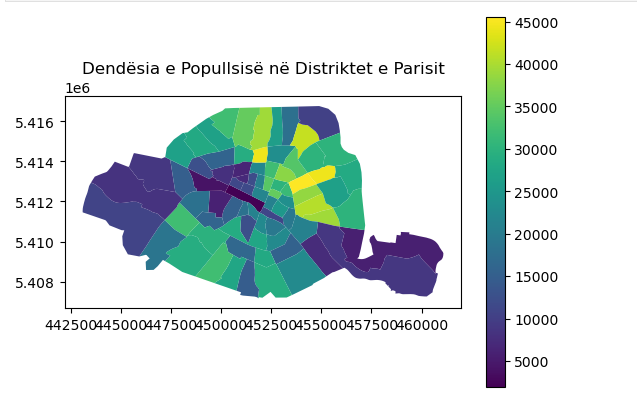
\includegraphics{./Figs/popdist.png}
\end{frame}

\begin{frame}{Shembull : Përdorimi i Funksionalitetit të Pandas:
Groupby}
\protect\hypertarget{shembull-puxebrdorimi-i-funksionalitetit-tuxeb-pandas-groupby}{}
\begin{itemize}
\item
  Në këtë ushtrim, do të përmbledhim një funksionalitet të zakonshëm:
  operacionin ``groupby''.
\item
  Mund të përdorni këtë operacion kur keni një kolonë që përmban grupe
  dhe dëshironi të llogaritni një statistikë për secilin grup.
\end{itemize}
\end{frame}

\begin{frame}[fragile]{Shembull : Përdorimi i Funksionalitetit të
Pandas: Groupby}
\protect\hypertarget{shembull-puxebrdorimi-i-funksionalitetit-tuxeb-pandas-groupby-1}{}
\begin{itemize}
\item
  Në metodën \texttt{groupby()}, kaloni kolonën që përmban grupet.
\item
  Në objektin që rezulton, mund të thërrisni metodën që dëshironi të
  llogaritni për secilin grup. Në këtë ushtrim, duam të dimë madhësinë e
  çdo grupi të tipit të restoranteve.
\end{itemize}
\end{frame}

\begin{frame}[fragile]{Përdorimi i \texttt{groupby()} për të grupuar dhe
llogaritur madhësinë e secilit grup}
\protect\hypertarget{puxebrdorimi-i-groupby-puxebr-tuxeb-grupuar-dhe-llogaritur-madhuxebsinuxeb-e-secilit-grup}{}
\AddToHookNext{env/Highlighting/begin}{\scriptsize}

\begin{Shaded}
\begin{Highlighting}[]
\CommentTok{\# Load the restaurants data}
\NormalTok{restaurants }\OperatorTok{=}\NormalTok{ geopandas.read\_file(}\StringTok{"data/gis/paris\_restaurants.csv"}\NormalTok{)}

\CommentTok{\# Grupojmë restorantet sipas llojit të restoranteve dhe llogarisim madhësinë e çdo grupi}
\NormalTok{type\_counts }\OperatorTok{=}\NormalTok{ restaurants.groupby(}\StringTok{\textquotesingle{}type\textquotesingle{}}\NormalTok{).size())}
\end{Highlighting}
\end{Shaded}

Kjo krijon një seri që tregon numrin e elementëve për secilin lloj
restoranti.
\end{frame}

\begin{frame}[fragile]{Printimi i Rezultatit}
\protect\hypertarget{printimi-i-rezultatit}{}
\AddToHookNext{env/Highlighting/begin}{\scriptsize}

\begin{Shaded}
\begin{Highlighting}[]
\CommentTok{\# Tregojmë serinë që përmban madhësinë e çdo grupi}
\BuiltInTok{print}\NormalTok{(type\_counts)}
\end{Highlighting}
\end{Shaded}

Kjo do të tregojë statistikat për secilin lloj restoranti, duke na dhënë
një ide të shpërndarjes së restoranteve sipas llojit.
\end{frame}

\begin{frame}{Shembull: Vizualizimi i Shtresave të Shumta}
\protect\hypertarget{shembull-vizualizimi-i-shtresave-tuxeb-shumta}{}
\begin{itemize}
\tightlist
\item
  Një funksionalitet tjetër tipik i pandas është filtrimi i një
  dataframe: marrja e një nën-grupi të rreshtave bazuar në një kusht (që
  gjeneron një maskë boolean).
\end{itemize}
\end{frame}

\begin{frame}[fragile]{Shembull: Vizualizimi i Shtresave të Shumta}
\protect\hypertarget{shembull-vizualizimi-i-shtresave-tuxeb-shumta-1}{}
\begin{itemize}
\item
  Në këtë ushtrim, do të marrim nën-grupin e të gjitha restoranteve
  afrikane dhe më pas do të krijojmë një grafik me shtresa të shumta.
\item
  Në një grafik të tillë, ne kombinojmë vizualizimin e disa
  GeoDataFrames në një figurë të vetme.
\item
  Për të shtuar një shtresë, mund të përdorim fjalën kyçe \texttt{ax} të
  metodës \texttt{plot()} të GeoDataFrame për t'i kaluar një objekt të
  boshtit të matplotlib.
\end{itemize}
\end{frame}

\begin{frame}[fragile]{Filtrimi për Restorantet Afrikane}
\protect\hypertarget{filtrimi-puxebr-restorantet-afrikane}{}
\AddToHookNext{env/Highlighting/begin}{\scriptsize}

\begin{Shaded}
\begin{Highlighting}[]
\CommentTok{\# Marrim nën{-}grupin e të gjitha rreshtave ku tipi është \textquotesingle{}African restaurant\textquotesingle{}}
\NormalTok{african\_restaurants }\OperatorTok{=}\NormalTok{ restaurants[restaurants[}\StringTok{\textquotesingle{}type\textquotesingle{}}\NormalTok{] }\OperatorTok{==} \StringTok{\textquotesingle{}African restaurant\textquotesingle{}}\NormalTok{]}
\end{Highlighting}
\end{Shaded}

Kjo krijon një nën-grup me vetëm restorantet afrikane.
\end{frame}

\hypertarget{hyrje-nuxeb-objektet-gjeografike-nuxeb-python}{%
\section{Hyrje në Objektet Gjeografike në
Python''}\label{hyrje-nuxeb-objektet-gjeografike-nuxeb-python}}

\begin{frame}{Prezantimi i Objekteve Gjeografike në Python}
\protect\hypertarget{prezantimi-i-objekteve-gjeografike-nuxeb-python}{}
\begin{itemize}
\item
  Tani do të mësojmë se si objektet gjeometrike (vektor) përfaqësohen në
  Python duke përdorur një bibliotekë të quajtur \textbf{shapely}.
\item
  Biblioteka \textbf{geopandas} përdor gjeometrinë \textbf{shapely} për
  të përfaqësuar karakteristikat gjeografike në të dhëna.
\end{itemize}
\end{frame}

\begin{frame}{Prezantimi i Objekteve Gjeografike në Python}
\protect\hypertarget{prezantimi-i-objekteve-gjeografike-nuxeb-python-1}{}
\begin{itemize}
\tightlist
\item
  Kuptimi i mënyrës se si funksionojnë këto objekte gjeometrike dhe se
  si mund të krijohen në Python është jashtëzakonisht i dobishëm, sepse
  këto objekte janë blloqet themelore që na lejojnë të bëjmë analizën e
  të dhënave gjeografike.
\end{itemize}
\end{frame}

\begin{frame}{Prezantimi i Objekteve Gjeografike në Python}
\protect\hypertarget{prezantimi-i-objekteve-gjeografike-nuxeb-python-2}{}
\begin{itemize}
\tightlist
\item
  \textbf{Shapely} përdor një bibliotekë C++ të quajtur \textbf{GEOS}
  për të ndërtuar gjeometritë, e cila është një nga bibliotekat
  standarde e softeve GIS si PostGIS ose QGIS.
\end{itemize}
\end{frame}

\begin{frame}{Krijimi i Gjeometrive të Pikave}
\protect\hypertarget{krijimi-i-gjeometrive-tuxeb-pikave}{}
\begin{itemize}
\item
  Kur krijojmë gjeometri me shapely, së pari duhet të importojmë klasën
  e objektit gjeometrik (siç është Point) që duam të krijojmë nga
  \textbf{shapely.geometry}.
\item
  \textbf{shapely.geometry} është gjeometria e cila përmban të gjitha
  llojet e mundshme të gjeometrisë.
\item
  Pas importimit të klasës \textbf{Point}, krijimi i një pike është i
  lehtë: ne thjesht kalojmë koordinatat x dhe y në klasën Point() (me
  një koordinatë të mundshme z) e cila do të krijojë pikën për ne:
\end{itemize}
\end{frame}

\begin{frame}[fragile]{Krijimi i Gjeometrive të Pikave}
\protect\hypertarget{krijimi-i-gjeometrive-tuxeb-pikave-1}{}
\AddToHookNext{env/Highlighting/begin}{\scriptsize}

\begin{Shaded}
\begin{Highlighting}[]
\CommentTok{\# Importimi i klasës Point nga shapely.geometry}
\ImportTok{from}\NormalTok{ shapely.geometry }\ImportTok{import}\NormalTok{ Point}

\CommentTok{\# Krijimi i gjeometrive të pikave}
\NormalTok{point }\OperatorTok{=}\NormalTok{ Point(}\FloatTok{2.2}\NormalTok{, }\FloatTok{4.2}\NormalTok{)  }\CommentTok{\# Për pikë 2D}
\NormalTok{point3D }\OperatorTok{=}\NormalTok{ Point(}\FloatTok{9.26}\NormalTok{, }\OperatorTok{{-}}\FloatTok{2.456}\NormalTok{, }\FloatTok{0.57}\NormalTok{)  }\CommentTok{\# Për pikë 3D}
\end{Highlighting}
\end{Shaded}
\end{frame}

\begin{frame}[fragile]{Ekstraktimi i Koordinatave të Pikave}
\protect\hypertarget{ekstraktimi-i-koordinatave-tuxeb-pikave}{}
\AddToHookNext{env/Highlighting/begin}{\scriptsize}

\begin{Shaded}
\begin{Highlighting}[]
\CommentTok{\# Ekstraktimi i koordinatave si listë}
\BuiltInTok{list}\NormalTok{(point.coords)  }\CommentTok{\# Kthen listën e koordinatave}
\CommentTok{\# Direkt nga atributet X dhe Y}
\BuiltInTok{print}\NormalTok{(point.x)  }\CommentTok{\# Koordinata X}
\BuiltInTok{print}\NormalTok{(point.y)  }\CommentTok{\# Koordinata Y}
\end{Highlighting}
\end{Shaded}
\end{frame}

\begin{frame}[fragile]{Krijimi i Gjeometrive LineString}
\protect\hypertarget{krijimi-i-gjeometrive-linestring}{}
\AddToHookNext{env/Highlighting/begin}{\scriptsize}

\begin{Shaded}
\begin{Highlighting}[]
\CommentTok{\# Importimi i klasave LineString dhe Point}
\ImportTok{from}\NormalTok{ shapely.geometry }\ImportTok{import}\NormalTok{ LineString, Point}

\CommentTok{\# Krijimi i gjeometrive të linjave}
\NormalTok{point1 }\OperatorTok{=}\NormalTok{ Point(}\FloatTok{2.2}\NormalTok{, }\FloatTok{4.2}\NormalTok{)}
\NormalTok{point2 }\OperatorTok{=}\NormalTok{ Point(}\FloatTok{7.2}\NormalTok{, }\OperatorTok{{-}}\FloatTok{25.1}\NormalTok{)}
\NormalTok{point3 }\OperatorTok{=}\NormalTok{ Point(}\FloatTok{9.26}\NormalTok{, }\OperatorTok{{-}}\FloatTok{2.456}\NormalTok{)}

\NormalTok{line }\OperatorTok{=}\NormalTok{ LineString([point1, point2, point3])}
\end{Highlighting}
\end{Shaded}

Linjat krijohen duke përdorur të paktën dy pika ose duke kaluar lista të
tupleve koordinatash.
\end{frame}

\begin{frame}[fragile]{Ekstraktimi i Koordinatave të LineString}
\protect\hypertarget{ekstraktimi-i-koordinatave-tuxeb-linestring}{}
\AddToHookNext{env/Highlighting/begin}{\scriptsize}

\begin{Shaded}
\begin{Highlighting}[]
\CommentTok{\# Ekstraktimi i koordinatave të LineString}
\BuiltInTok{list}\NormalTok{(line.coords)  }\CommentTok{\# Kthen listën e koordinatave të linjave}
\end{Highlighting}
\end{Shaded}

Kjo na jep një listë me çiftet e koordinatave (x, y).
\end{frame}

\begin{frame}[fragile]{Krijimi i Gjeometrive Polygon}
\protect\hypertarget{krijimi-i-gjeometrive-polygon}{}
\AddToHookNext{env/Highlighting/begin}{\scriptsize}

\begin{Shaded}
\begin{Highlighting}[]
\CommentTok{\# Importimi i klasës Polygon}
\ImportTok{from}\NormalTok{ shapely.geometry }\ImportTok{import}\NormalTok{ Polygon}

\CommentTok{\# Krijimi i gjeometrive të poligoneve}
\NormalTok{poly }\OperatorTok{=}\NormalTok{ Polygon([point1, point2, point3])  }\CommentTok{\# Poligoni me tre pika}
\end{Highlighting}
\end{Shaded}

Poligonet krijohen me të paktën tre pika ose një listë të koordinatave.
\end{frame}

\begin{frame}[fragile]{Ekstraktimi i Informacionit nga Polygon}
\protect\hypertarget{ekstraktimi-i-informacionit-nga-polygon}{}
\AddToHookNext{env/Highlighting/begin}{\scriptsize}

\begin{Shaded}
\begin{Highlighting}[]
\CommentTok{\# Informacioni për Polygon}
\BuiltInTok{print}\NormalTok{(}\StringTok{"Polygon centroid: "}\NormalTok{, poly.centroid)  }\CommentTok{\# Gjen qendrën e poligonit}
\BuiltInTok{print}\NormalTok{(}\StringTok{"Polygon Area: "}\NormalTok{, poly.area)  }\CommentTok{\# Sipërfaqja e poligonit}
\end{Highlighting}
\end{Shaded}

Shumë funksione mund të nxirren direkt nga Polygon, si qendra (centroid)
dhe sipërfaqja.
\end{frame}

\begin{frame}[fragile]{Krijimi i Poligonëve me Hapësirë Boshe (Holes)}
\protect\hypertarget{krijimi-i-poligonuxebve-me-hapuxebsiruxeb-boshe-holes}{}
\AddToHookNext{env/Highlighting/begin}{\scriptsize}

\begin{Shaded}
\begin{Highlighting}[]
\CommentTok{\# Definimi i unazës së jashtme dhe së brendshme për të krijuar një poligon me hapësirë boshe}
\NormalTok{exterior }\OperatorTok{=}\NormalTok{ [(}\OperatorTok{{-}}\DecValTok{180}\NormalTok{, }\DecValTok{90}\NormalTok{), (}\OperatorTok{{-}}\DecValTok{180}\NormalTok{, }\OperatorTok{{-}}\DecValTok{90}\NormalTok{), (}\DecValTok{180}\NormalTok{, }\OperatorTok{{-}}\DecValTok{90}\NormalTok{), (}\DecValTok{180}\NormalTok{, }\DecValTok{90}\NormalTok{)]  }\CommentTok{\# Unaza e jashtme}
\NormalTok{hole }\OperatorTok{=}\NormalTok{ [[(}\OperatorTok{{-}}\DecValTok{170}\NormalTok{, }\DecValTok{80}\NormalTok{), (}\OperatorTok{{-}}\DecValTok{170}\NormalTok{, }\OperatorTok{{-}}\DecValTok{80}\NormalTok{), (}\DecValTok{170}\NormalTok{, }\OperatorTok{{-}}\DecValTok{80}\NormalTok{), (}\DecValTok{170}\NormalTok{, }\DecValTok{80}\NormalTok{)]]  }\CommentTok{\# Unaza e brendshme}

\NormalTok{poly\_with\_hole }\OperatorTok{=}\NormalTok{ Polygon(shell}\OperatorTok{=}\NormalTok{exterior, holes}\OperatorTok{=}\NormalTok{hole)  }\CommentTok{\# Krijimi i poligonit me hapësirë boshe}
\end{Highlighting}
\end{Shaded}

Poligonet mund të kenë hapësira bosh duke përdorur parametrat shell për
unazën e jashtme dhe holes për ato të brendshme.
\end{frame}

\begin{frame}[fragile]{Krijimi i Gjeometrive MultiPoint,
MultiLineString, dhe MultiPolygon}
\protect\hypertarget{krijimi-i-gjeometrive-multipoint-multilinestring-dhe-multipolygon}{}
\AddToHookNext{env/Highlighting/begin}{\scriptsize}

\begin{Shaded}
\begin{Highlighting}[]
\CommentTok{\# Importimi i klasave MultiPoint, MultiLineString, dhe MultiPolygon}
\ImportTok{from}\NormalTok{ shapely.geometry }\ImportTok{import}\NormalTok{ MultiPoint, MultiLineString, MultiPolygon}

\CommentTok{\# Krijimi i MultiPoint}
\NormalTok{multipoint }\OperatorTok{=}\NormalTok{ MultiPoint([Point(}\DecValTok{2}\NormalTok{, }\DecValTok{2}\NormalTok{), Point(}\DecValTok{3}\NormalTok{, }\DecValTok{3}\NormalTok{)])  }\CommentTok{\# Koleksion i pikave}

\CommentTok{\# Krijimi i MultiLineString}
\NormalTok{multiline }\OperatorTok{=}\NormalTok{ MultiLineString([}
\NormalTok{    LineString([(}\DecValTok{2}\NormalTok{, }\DecValTok{2}\NormalTok{), (}\DecValTok{3}\NormalTok{, }\DecValTok{3}\NormalTok{)]),}
\NormalTok{    LineString([(}\DecValTok{4}\NormalTok{, }\DecValTok{3}\NormalTok{), (}\DecValTok{6}\NormalTok{, }\DecValTok{4}\NormalTok{)])}
\NormalTok{])  }\CommentTok{\# Koleksion i linjave}

\CommentTok{\# Krijimi i MultiPolygon}
\NormalTok{multipoly }\OperatorTok{=}\NormalTok{ MultiPolygon([}
\NormalTok{    Polygon([(}\DecValTok{0}\NormalTok{, }\DecValTok{0}\NormalTok{), (}\DecValTok{0}\NormalTok{, }\DecValTok{4}\NormalTok{), (}\DecValTok{4}\NormalTok{, }\DecValTok{4}\NormalTok{)]),}
\NormalTok{    Polygon([(}\DecValTok{6}\NormalTok{, }\DecValTok{6}\NormalTok{), (}\DecValTok{6}\NormalTok{, }\DecValTok{12}\NormalTok{), (}\DecValTok{12}\NormalTok{, }\DecValTok{12}\NormalTok{)])}
\NormalTok{])  }\CommentTok{\# Koleksion i poligoneve}
\end{Highlighting}
\end{Shaded}

Versionet ``Multi'' të gjeometrive lejojnë përfaqësimin e koleksioneve
të shumta me pika, linja, ose poligone.
\end{frame}

\end{document}
